\section{Beyond graphene: TMD nanoribbons}
\label{sec:state}

\ac{2D} materials have steadily been drawing the attention of the community since graphene was experimentally isolated from a graphite sample by mechanical exfoliation, yielding a system constituted by a single layer of atoms (Figure \ref{fig:graphene}, left).
Since then, numerous studies have been made due to the promising properties of these materials, and the interesting as-yet-unseen phenomena occurring within them, for example: unconventional quantum Hall effect, absence of localization, and electrons behaving like massless relativistic particles (Figure \ref{fig:graphene}, right), providing a bridge between condensed matter physics and quantum electrodynamics \cite{katsnelson_graphene:_2007}.
In spite of its undeniable potential, graphene has some shortcomings.
This motivated the community to study other more complex graphene-like materials, which could have desirable properties.

\begin{figure}[H]
\hspace{1cm}

\includegraphics[width = 3.6cm]{Introduction/graphene.png}
\hspace{3cm}
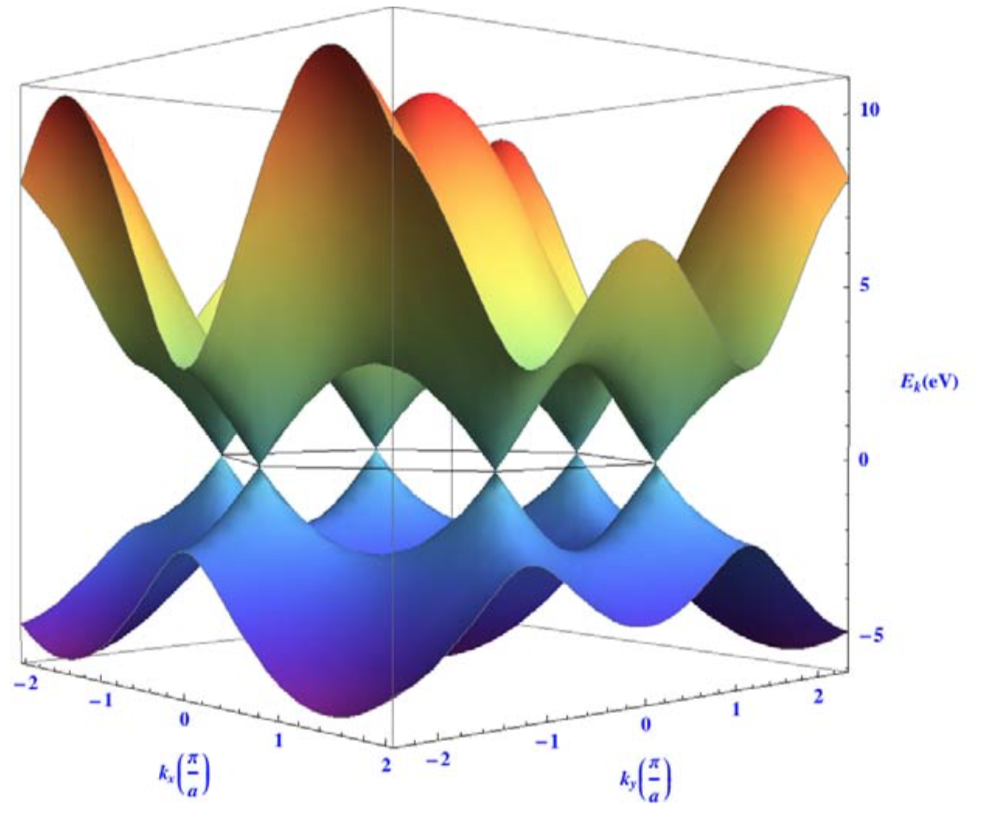
\includegraphics[width = 6.5cm]{Introduction/disp_rel.png}
\caption[Graphene monolayer; graphene's dispersion relation.]{Left: \acf{AFM} picture of a graphene monolayer. The black area is a substrate used for fabrication purposes. The dark orange area is a monolayer of graphene. Right: Dispersion relation of graphene. The black line represents the Fermi energy. Close to it, the dispersion relation is linear, corresponding to massless excitations (taken from \cite{noauthor_nobel_nodate}). }
\label{fig:graphene}
\end{figure}	

\acp{TMD} are a novel member of the \ac{2D} materials family \cite{wang_electronics_2012, roldan_electronic_2014, xu_spin_2014}.
They have been attracting interest because they seem to overcome some of the drawbacks of graphene in technological applications.
For example, monolayer graphene is gapless, while its bilayer counterpart has only a tunable, but small gap of the order of a tenth of an $eV$.
Contrastingly, \acp{TMD} have an intrinsic gap in excess of $1 \, eV$, being more promising in designing, for example, transistors.
Hole-doped \acp{TMD} are expected to show topological superconductivity \cite{hsu_topological_2017}, while the superconducting phase of graphene has been predicted, but is not easily attained.
Superconductivity in graphene-like \ac{2D} materials is important because it could boost high speed nanoelectronics.
Moreover, the presence of transition metal atoms in \acp{TMD} suggests the possibility of magnetic ordering \cite{braz_valley_2017}, which could be very relevant in nanospintronics applications.
Both topological superconductivity and magnetic ordering arise due to the effect of strong electron correlations.
Thus, to investigate these properties of \acp{TMD} reliably, we need a computational method that is robust enough to capture the effects of electron interactions.

A particularly promising type of \acs{2D}  nanostructures are nanoribbons.
A nanoribbon consists of a \ac{2D} layer that can be regarded as infinitely long on one direction, but not on the other (Figure \ref{fig:fabrication}), so that edge states become relevant, and can be controlled to yield interesting properties.
For simulation purposes, it is natural to assume translational invariance along the ribbon's longitudinal direction, and use \acp{PBC}.
On the other direction, we use \acp{OBC}, effectively considering zigzag edges (Figure \ref{fig:nanoribbons}, left).

\begin{figure}[H]
\centering
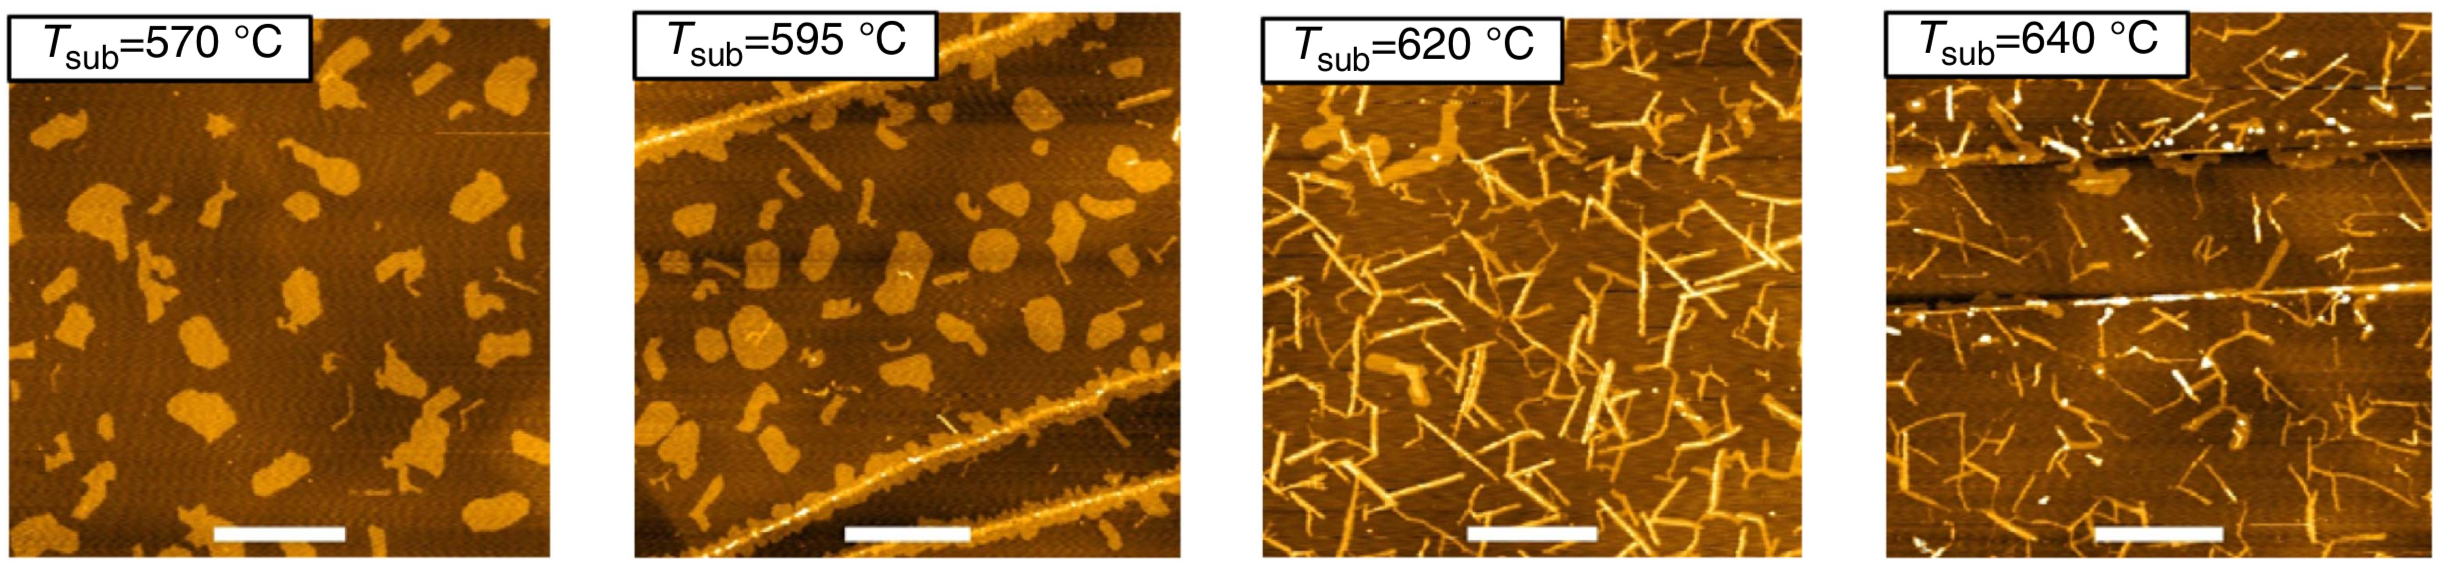
\includegraphics[scale = 0.32]{Introduction/nanoribbons}
\caption[Fabrication of \ac{TMD} nanoribbons]{Fabrication of \ac{TMD} nanoribbons. From left to right, we see \ac{AFM} images showing the appeareance of nanostructures ranging from \ac{2D} nanoislands to nanoribbons, as the temperature of the substrate is increased. The nanoribbons are grown by taking advantage of the temperature dependence of shape transformations occuring during the nonequilibrium growth of this kind of surface-based nanostructures. (taken from \cite{chen_fabrication_2017})}
\label{fig:fabrication}
\end{figure}

\begin{figure}[H]
\centering
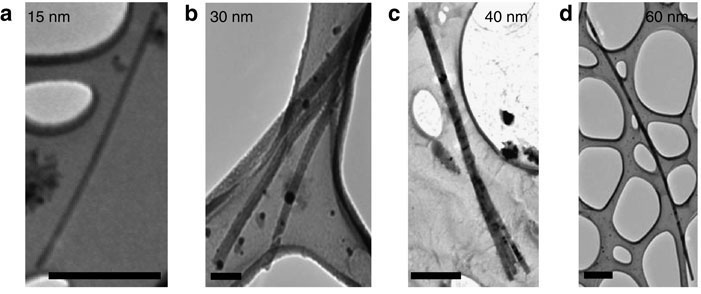
\includegraphics[scale = 0.4]{Introduction/grapheneNanoribbons.jpg}
\caption[(TEM) images of graphene nanoribbons.]{(a) to (d) - Transmission electron microscopy (TEM) images of graphene nanoribbons (GNRs) of widths 15, 30, 40, and 60 $nm$, respectively (adapted from \cite{mohanty_nanotomy-based_2012} ).}
\label{fig:fabrication}
\end{figure}
   
A high density of low-energy electronic states is localized at the zigzag edges, decaying quickly in the bulk, which suggests the possibility of magnetic ordering.
In fact, a mean field solution of the Hubbard model for a graphene nanoribbon shows that magnetic moments are localized at the edges \cite{yazyev_emergence_2010} (Figure \ref{fig:nanoribbons}, right).
QMC has been used to investigate edge-state magnetism beyond mean field in graphene \cite{feldner_dynamical_2011, golor_quantum_2013, cheng_strain-induced_2015, raczkowski_interplay_2017, yang_strain-tuning_2017}.
However, edge-state magnetism in \acp{TMD} remains unexplored \cite{davelou_nanoribbon_2017}, and we would like to investigate, for example, whether edge-state magnetism is stabilized at finite temperature in \acp{TMDNR}.
 
\begin{figure}[H]
\vspace{-0.5cm}
\hspace{0.2cm}
\begin{minipage}[c]{0.1\textwidth}
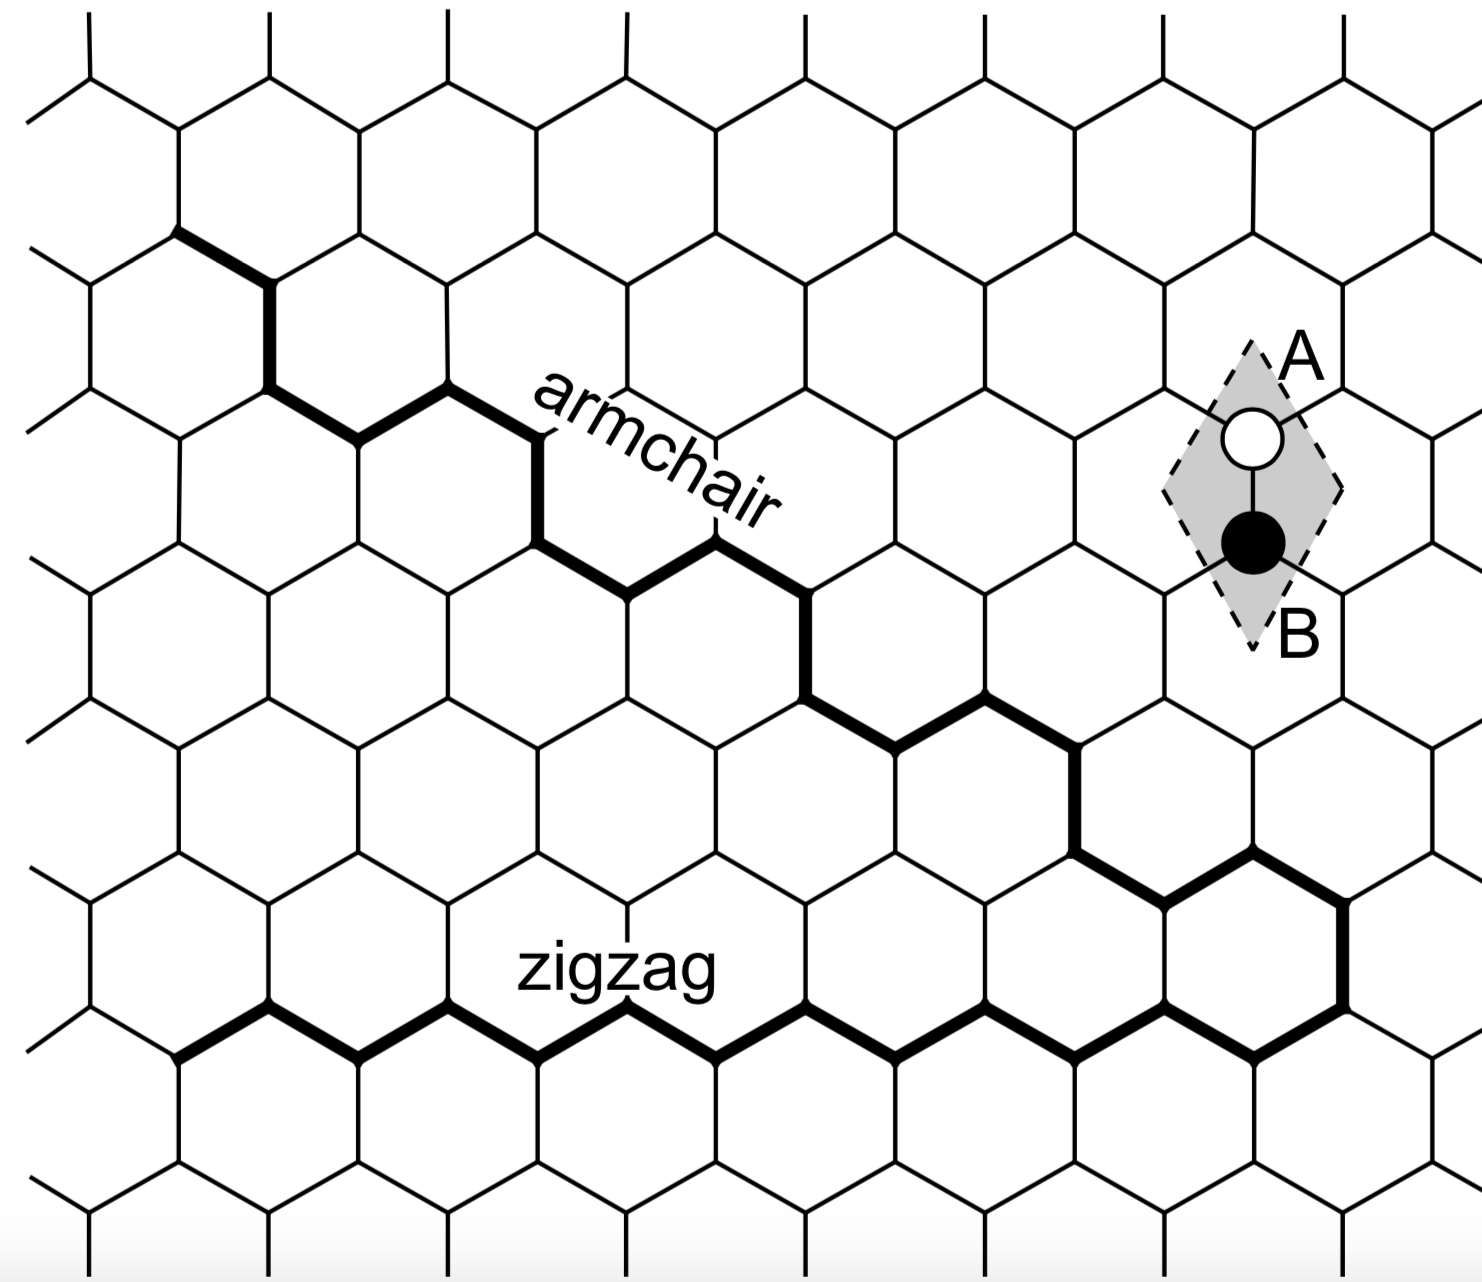
\includegraphics[scale = 0.21]{Introduction/zigzag}
\end{minipage} \hspace{4.2cm}
\begin{minipage}[c]{0.1\textwidth}
\vspace{0.3cm}
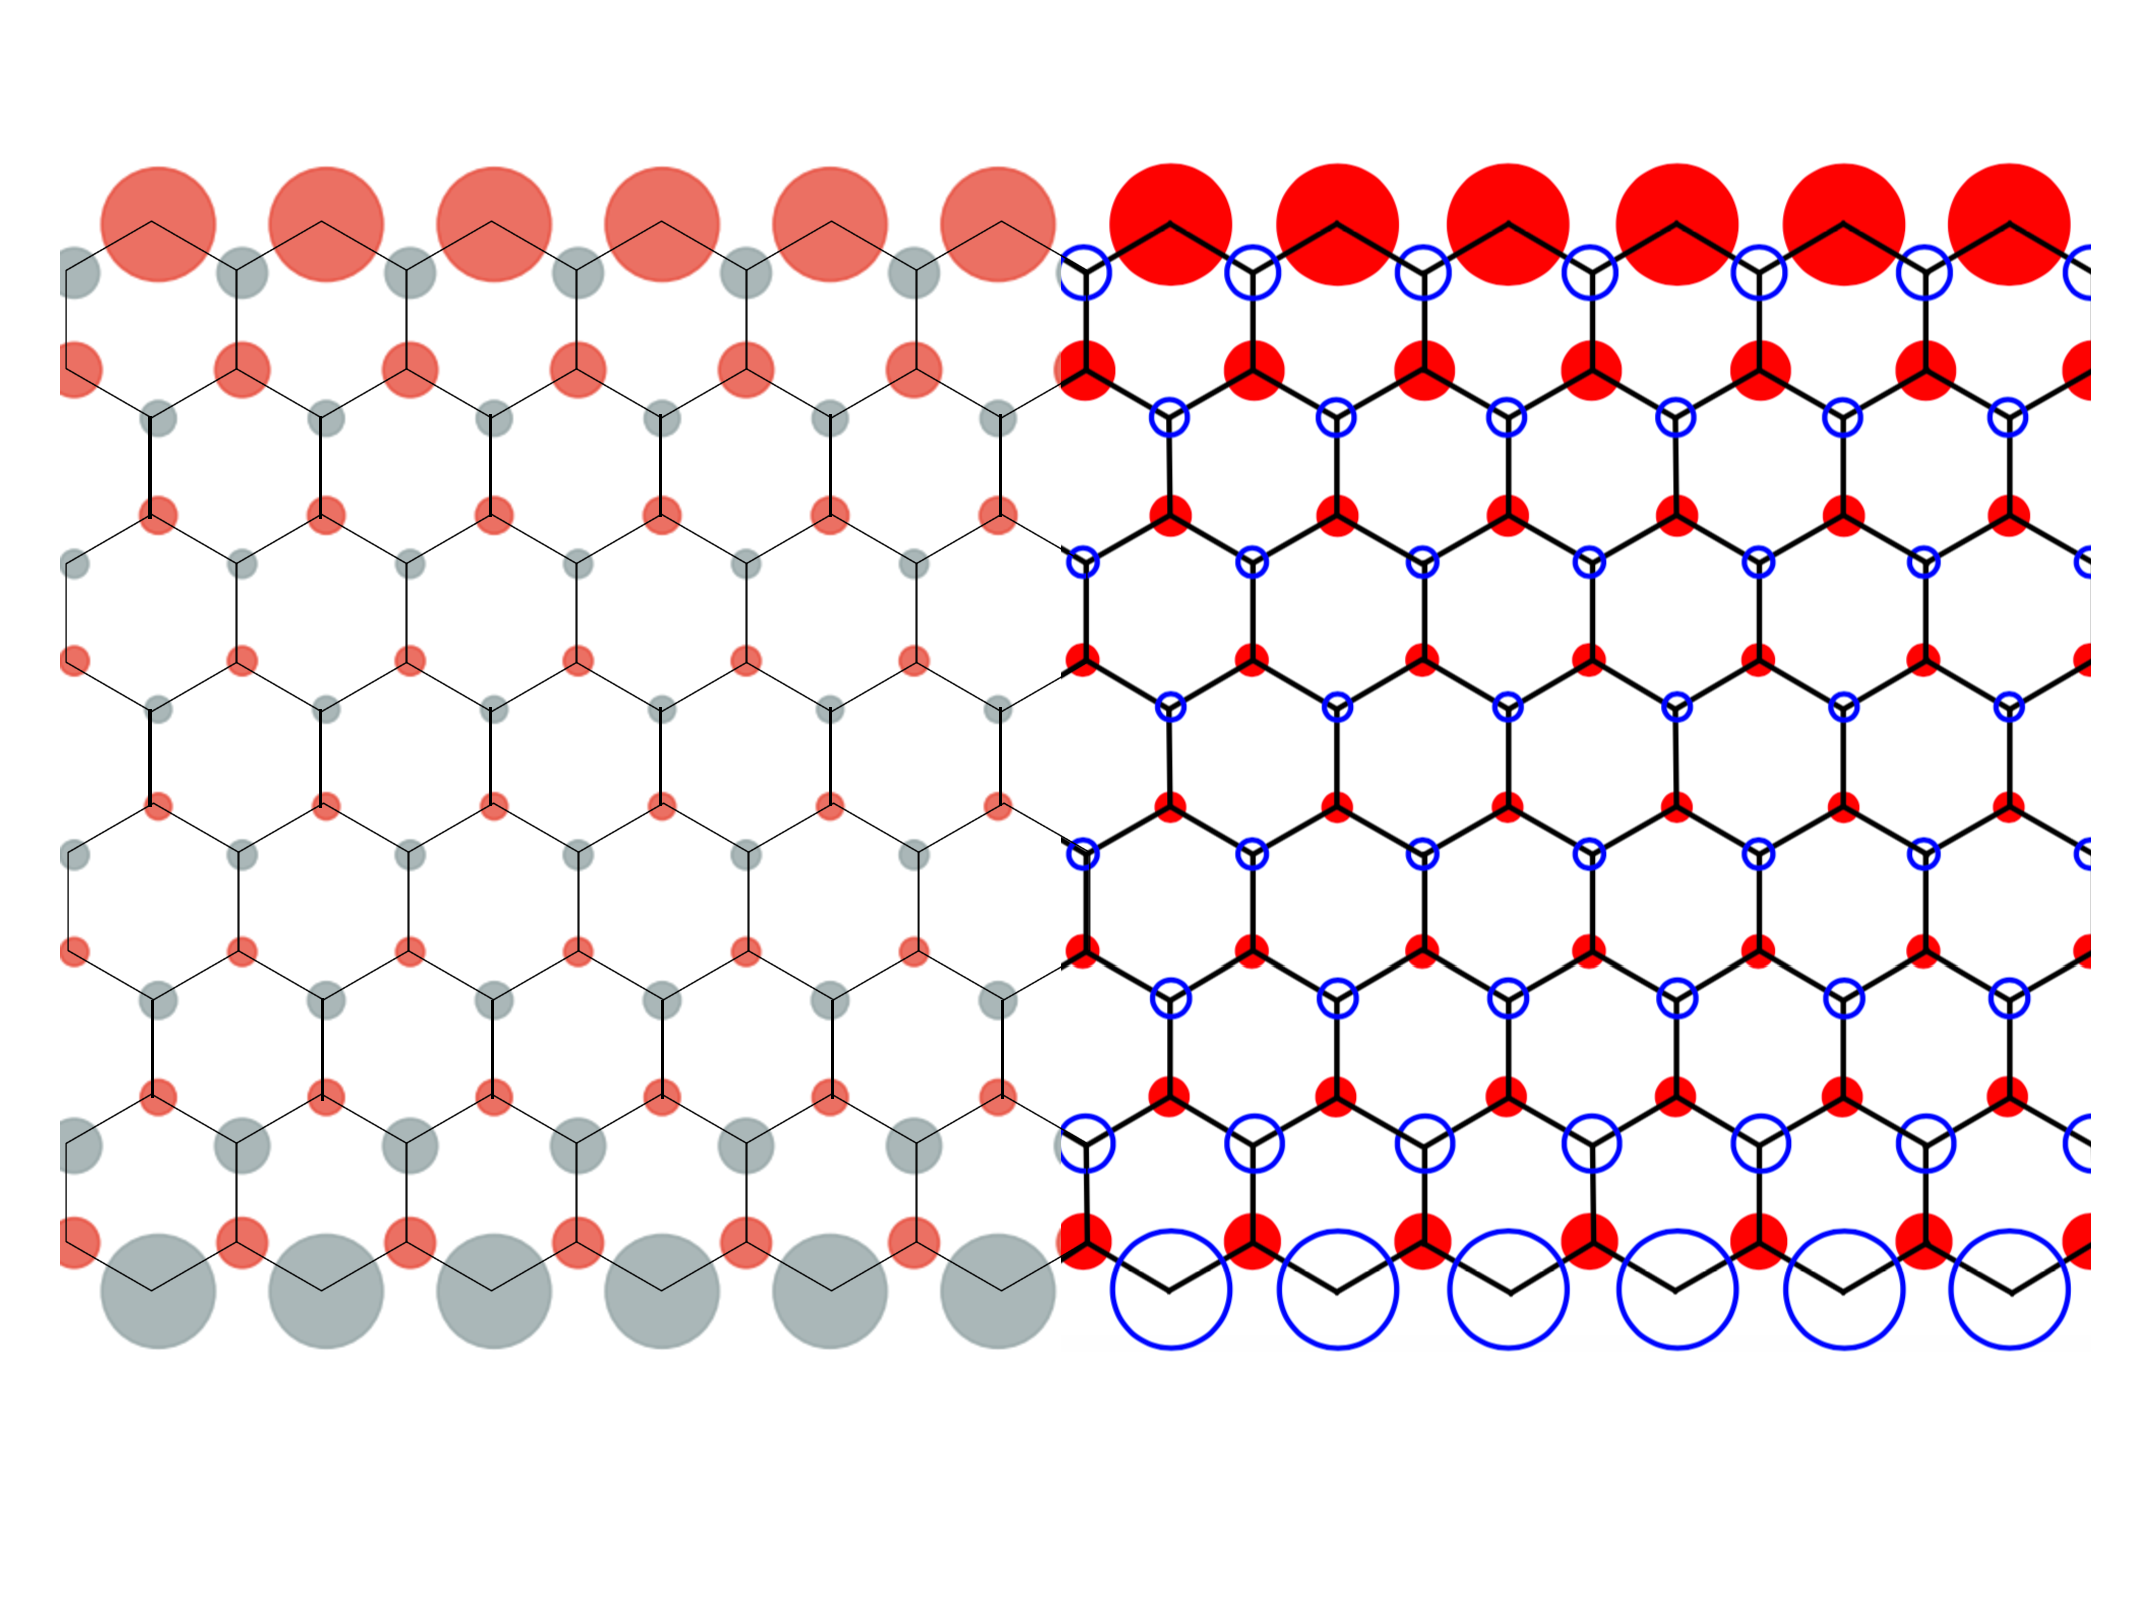
\includegraphics[scale = 0.24]{Introduction/comparisonMF.pdf}
\end{minipage}
\vspace{-0.5cm}
 \caption[Zigzag edges of a nanoribbon and magnetism.]{Left: Two possible terminations of a \ac{TMD} nanoribbon condensing in a honeycomb lattice.
Right: Local magnetic moments tend to develop on the zig zag edges.
The area of the circles corresponds to the magnitude of the magnetic moment.
The red circles corresponds to the spin up density, and the blue ones to the spin down density.
The particular arrangement of the electronic edge states leads to an \ac{AF} ground state (opposite edges with opposite magnetic moment). The results on the right part of the picture are taken from \cite{yazyev_emergence_2010}, while the left part corresponds to our original results clearly reproducing the ones on the literature). \label{fig:nanoribbons}}
\end{figure}

While the zigzag graphene nanoribbon antiferromagnetic ground state is semiconducting, a state with interedge ferromagnetic orientation is a metal.
An example of an application based on the switching between the two states is a magnetorresistive sensor.
This device allows switching between low and high-resistance configurations, corresponding, respectively, to parallel, and antiparallel configurations of ferromagnetic leads at the ends of a nanoribbon.
An analogous form of edge-state magnetism, as is observed in graphene nanoribbons, for \acp{TMDNR}, could yield similarly innovative applications.